\documentclass[12pt]{article}

% Packages 
\usepackage{amsmath}
\usepackage{amssymb}
\usepackage{datetime}
\usepackage{graphicx}
\usepackage{listings}

\graphicspath{{./images/}}

\newdate{date}{21}{03}{2022}
\title{
    Assignment B

    \large{
        ME EN 6240 Advanced Mechatronics
    }  
}
    
\author{
        Ryan Dalby
}
\date{\displaydate{date}}


\begin{document}
\maketitle

\section*{Exercise 1}
Note that subscript 1 implies the path where the 100$\Omega$ resistor and 0.1F capacitor are in series.
\begin{enumerate}
    \item[a.]
    $I_1 = \frac{(5-0)V}{100\Omega} = 0.05 A$

    $I_2 = \frac{(5-3)V}{10\Omega} = 0.2 A$

    \item[b.]
    $\dot{V}_c = I_c \frac{1}{C} = \frac{I_1}{C} = \frac{0.05}{0.1} = 0.5 V/s$
    % Need resistor before capacitor because current to resistor has to be limited in a way due to physical limits of specification of the capacitor

    \item[c.]
    \begin{enumerate}
        % At steady state
        \item[i.]
        $V_c = 5V$
        \item[ii.]
        $E_c = \frac{1}{2}CV^2 = 0.5*0.1*5^2 = 1.25 J$
        \item[iii.]
        At steady-state the battery is being discharged because current still flows the direction the battery would cause it to flow if it was by itself.
        $P = VI = 3 \frac{(5-3)}{10} = (3) (0.2) = 0.6 W$
        \item[iv.]
        At steady-state the battery is being discharged because current still flows the direction the battery would cause it to flow if it was by itself.
        $P = VI = (5) (0.2) = 1 W$
    
        % $P_{loss} = I^2 R = VI = 0.4$ 
    \end{enumerate}

    \item[d.]
    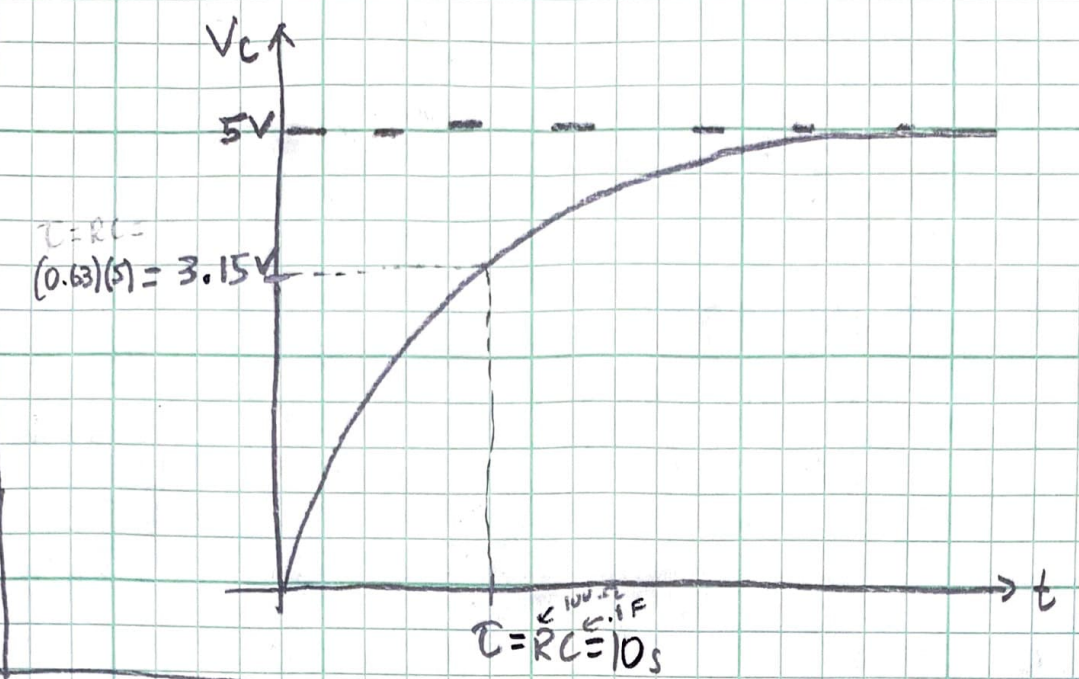
\includegraphics[width=4.8in]{1d.png}
    % $\dot{V}_c = \frac{5 - V_c}{RC}$
\end{enumerate}

\section*{Exercise 2}
% No current until around 0.7 V(typically) then steps up like step function there
% Diodes are directional
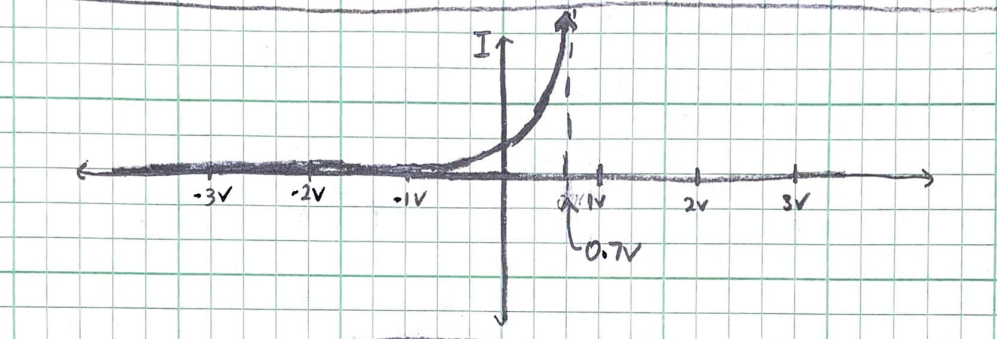
\includegraphics[width=5.2in]{2.png}

\section*{Exercise 3}
\begin{enumerate}
    \item[a.]
    % At steady state
    $V_L = 0V$
    $V_R = 10V$
    $I_1 = \frac{10V}{50\Omega} = 0.2A$

    \item[b.]
    % At steady state
    $V_{diode} = 0V - 10V = -10V$
    $I_2 = 0A$

    \item[c.]
    $E_L = \frac{1}{2} L I^2 = (0.5)(2)(0.2)^2 = 0.04 J$

    \item[d.]
    % Switch is opened, instant after
    \begin{enumerate}
        \item[i.] 
        $I_1 = 0.2 A$
    \end{enumerate}
    \item[e.]
    $I_2 = -0.2 A$

    \item[f.]
    $V_A = -0.7$

    \item[g.]
    $\frac{\mathrm{d} I_1}{\mathrm{d} t} = \frac{V_L}{L} = \frac{-10.7}{2} = -5.35 A/s$

    \item[h.]
    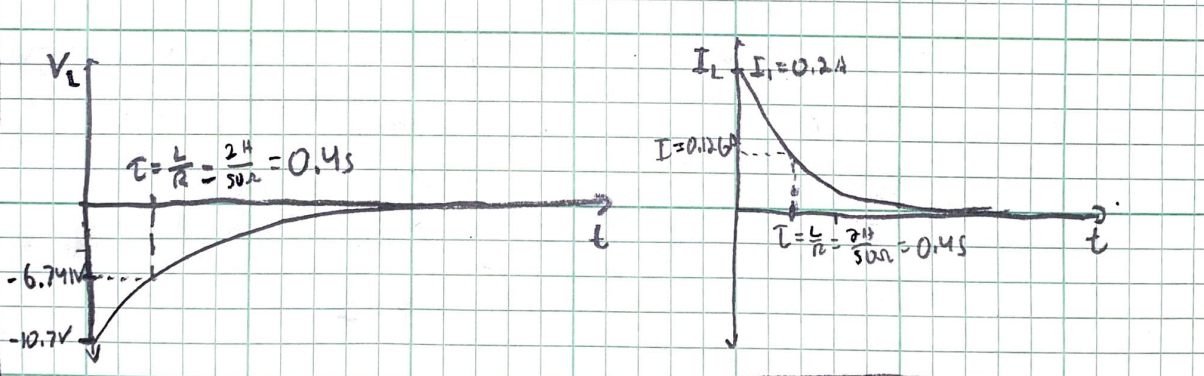
\includegraphics[width=4.8in]{3h.png}

    % Diodes are very useful for preventing "infinite" inductance voltages on sudden current changes by giving a path for current to flow after the change in current in a way that prevents large voltages from causing energy from being discharged outside of circuit
\end{enumerate}

\section*{Exercise 4}
{\setlength{\parindent}{0cm}
For off:

$V_{in} < V_{be,on}$

For saturated:

$V_{ce} = V_c - V_e = V_s - V_e \ge V_{ce,sat}$

$V_e = I_e R_2$

$I_e = (1+\beta) I_b$

$V_b = V_{be,on} + V_e = V_{be,on} + I_e R_2$

$I_b = \frac{V_{in} - (V_{be,on} + I_e R_2)}{R_1}$

$V_{ce} = V_s - V_e = V_s - \frac{R_2 (1+\beta) (V_{in} - V_{be,on})}{R_1 + R_2(1+\beta)} \ge V_{ce,sat}$

$V_{in} \le - \frac{V_{ce,sat} R_1 + R_2(1+\beta)}{R_2 (1+\beta)} - V_s + V_{be,on}$
}

\section*{Exercise 5}
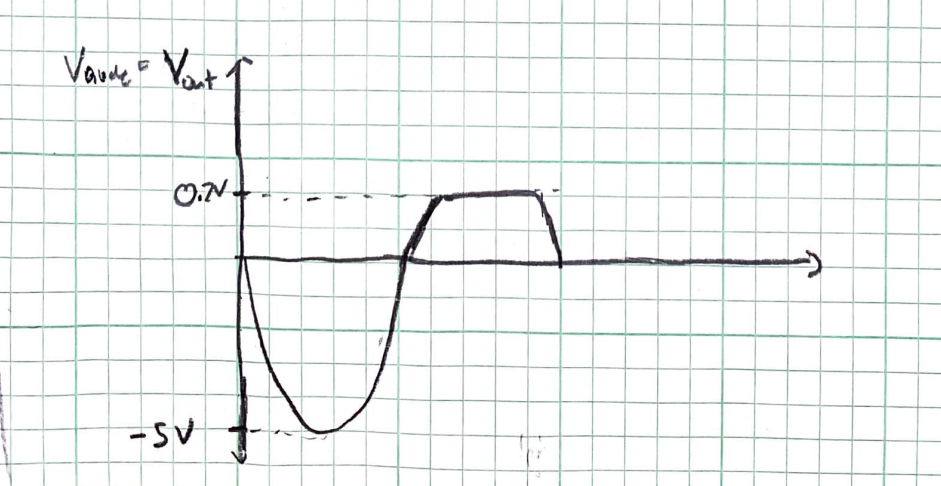
\includegraphics[width=5.2in]{5.png}

\section*{Exercise 6}
{\setlength{\parindent}{0cm}
$V_n = V_p = 0 V$

$V_{out} = R_2 I_2$

$I_2 = -I_{R_1} -I_c$

$I_{R_1} = \frac{V_1}{R_1}$

$I_c = C \dot{V_2}$

$V_{out} = R_2 (-\frac{V_1}{R_1} - C \dot{V_2})$
}


\section*{Exercise 7}
{\setlength{\parindent}{0cm}
$V_p = V_n$

$V_p = V_2 - I_2 R = V_n$

$I_1 = I_c = \frac{V_1 - V_2 - I_2 R}{R}$

$\dot{V_c} = \frac{I_c}{C} = \dot{V_n} - \dot{V_{out}}$

$\dot{V_n} = \dot{V_2} - \dot{I_2} R$

$\dot{V_{out}} = \dot{V_2} - \dot{I_2} R - \frac{V_1 - V_2 - I_2 R}{RC}$
}
\end{document}